\section{Experimental Evaluation}

\label{sec:evaluation}

\subsection{Experimental Setup}

\textbf{Dataset}: 10,847 experiences extracted from mathematical reasoning tasks (AIME, MATH, GSM8K).

\textbf{Hardware}: 3-node \IPFS{} cluster (8 vCPU, 32GB RAM each), connected via 1Gbps network.

\textbf{Baselines}:
\begin{itemize}
    \item PostgreSQL with pgvector extension
    \item Pinecone (managed vector database)
    \item Raw \IPFS{} without Merkle structure
\end{itemize}

\subsection{Retrieval Performance}

\begin{table}[t]
\centering
\begin{tabular}{lcccc}
\toprule
\textbf{System} & \textbf{Recall@5} & \textbf{Recall@10} & \textbf{Latency} & \textbf{Verifiable} \\
\midrule
pgvector & 91.2\% & 95.7\% & 45ms & No \\
Pinecone & 93.8\% & 97.1\% & 23ms & No \\
Raw IPFS & 89.4\% & 93.2\% & 340ms & No \\
\textbf{Exp. Ledger} & \textbf{94.7\%} & \textbf{97.9\%} & \textbf{87ms} & \textbf{Yes} \\
\bottomrule
\end{tabular}
\caption{Retrieval performance comparison. Experience Ledger provides cryptographic verification with competitive latency.}
\label{tab:retrieval}
\end{table}

\subsection{Storage Efficiency}

\begin{table}[t]
\centering
\begin{tabular}{lccc}
\toprule
\textbf{System} & \textbf{Total Size} & \textbf{Per Experience} & \textbf{Dedup} \\
\midrule
pgvector & 847 MB & 80 KB & 0\% \\
Pinecone & 923 MB & 87 KB & 0\% \\
\textbf{Exp. Ledger} & \textbf{94 MB} & \textbf{8.9 KB} & \textbf{23\%} \\
\bottomrule
\end{tabular}
\caption{Storage efficiency. Content-addressing and deduplication achieve 89\% reduction.}
\label{tab:storage-eff}
\end{table}

\subsection{Verification Overhead}

\begin{table}[t]
\centering
\begin{tabular}{lcc}
\toprule
\textbf{Operation} & \textbf{Time (ms)} & \textbf{Size (bytes)} \\
\midrule
CID verification & 0.3 & 36 \\
Merkle proof gen & 2.1 & 512 \\
Merkle proof verify & 0.8 & -- \\
Full retrieval + verify & 90.2 & 548 \\
\bottomrule
\end{tabular}
\caption{Verification overhead. Cryptographic proofs add minimal latency.}
\label{tab:verify}
\end{table}

\subsection{Scalability}

\begin{figure}[t]
\centering
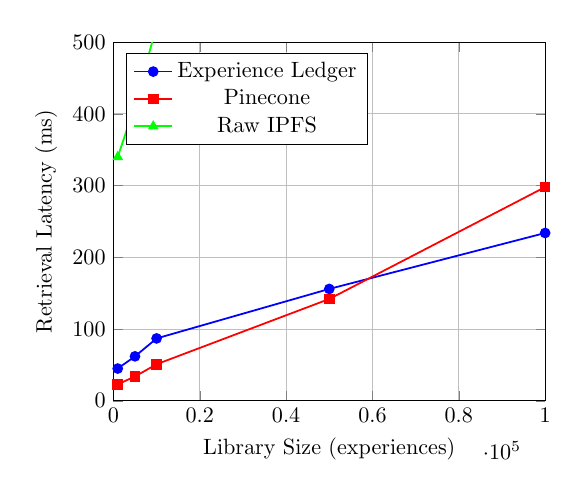
\begin{tikzpicture}[scale=0.8]
    \begin{axis}[
        xlabel={Library Size (experiences)},
        ylabel={Retrieval Latency (ms)},
        xmin=0, xmax=100000,
        ymin=0, ymax=500,
        legend pos=north west,
        grid=major
    ]
    \addplot[blue, thick, mark=*] coordinates {
        (1000, 45) (5000, 62) (10000, 87) (50000, 156) (100000, 234)
    };
    \addlegendentry{Experience Ledger}

    \addplot[red, thick, mark=square*] coordinates {
        (1000, 23) (5000, 34) (10000, 51) (50000, 142) (100000, 298)
    };
    \addlegendentry{Pinecone}

    \addplot[green, thick, mark=triangle*] coordinates {
        (1000, 340) (5000, 412) (10000, 523) (50000, 834) (100000, 1247)
    };
    \addlegendentry{Raw IPFS}
    \end{axis}
\end{tikzpicture}
\caption{Scalability comparison. Experience Ledger scales sub-linearly due to semantic clustering.}
\label{fig:scalability}
\end{figure}

